
%%
%% This .tex file is for use with BibLaTeX.
%%
%% As of Spring 2023, the School of Graduate Studies requires some minimum accessibility requirements for all electronic theses. Accessibility is difficult to produce with LaTeX on the front end, but fortunately it is quite easy to meet the requirements on the back end using Adobe (not Adobe Reader). Simply download the PDF of your thesis and follow this guide: https://case.edu/gradstudies/sites/case.edu.gradstudies/files/2023-02/CWRU%20Thesis%20and%20Dissertation%20Accessiblity%20Guide_0.pdf
%%%%%%%%%%%%

\documentclass[12pt]{cwru_thesis}
\usepackage[hyphens]{url}
\usepackage{indentfirst}
\usepackage{lipsum}
\usepackage{tabularx}
\usepackage{graphicx}
\usepackage{hyperref}
\usepackage{float}
\hypersetup{colorlinks=true, linkcolor=black, filecolor=black, urlcolor=black, citecolor=black}
\urlstyle{same}
% \usepackage[acronym,toc]{glossaries}
\usepackage[intoc]{nomencl}
\renewcommand{\nomname}{List of Symbols}

\usepackage{mathptmx}
\usepackage[T1]{fontenc}
\usepackage[utf8]{inputenc}
\usepackage{amsfonts, amsmath, amsthm, amssymb}
\usepackage{xstring}

\newcommand{\dif}{\mathrm{d}}
\newcommand{\Dif}{\mathrm{D}}
\renewcommand{\vec}[1]{\ensuremath{\underline{#1}}}
\newcommand{\grad}{\underline{\nabla}}
\newcommand{\curl}{\underline{\nabla} \times}
\newcommand{\lap}{\underline{\nabla}^2}
\renewcommand{\div}{\underline{\nabla} \cdot}
\newcommand{\paren}[1]{\left( {#1} \right)}
\newcommand{\norm}[1]{\lVert#1\rVert}

\usepackage[backend=biber, style=alphabetic, sorting=none, maxalphanames=4, maxbibnames=6]{biblatex}

% Custom label format
\DeclareLabelalphaTemplate{
  \labelelement{
    \field[final]{shorthand}
    \field{label}
    \field[strwidth=3, strside=left, ifnames=1]{labelname}
    \field[strwidth=1, strside=left, ifnames=2]{labelname}
    \field[strwidth=1, strside=left, ifnames=3]{labelname}
    \field[strwidth=1, strside=left, ifnames=4]{labelname}
    \field[strwidth=1, strside=left, ifnames=5]{labelname}
    \field[strwidth=1, strside=left, ifnames=6]{labelname}
  }
  \labelelement{
    \field[strwidth=2,strside=right]{year}
  }
}

% Custom label alpha for more than three authors
\renewcommand*{\labelalphaothers}{\textsuperscript{+}}

% Apply bold and uppercase formatting to the entire citation label
\DeclareFieldFormat{labelalpha}{\textbf{\MakeUppercase{#1}}}
\DeclareFieldFormat{extraalpha}{\textbf{\MakeUppercase{\mknumalph{#1}}}}

\addbibresource{example.bib}




% \makeglossaries
%%%%%%%%%%%%%%%%%%%%%%%%%%%%%%%%%%%%%%%%%%%%%%%%%%%%%%%%%%%%%%%%%%%%%%%%%%%%%%%%%%%%%%%
%Glossary entries


%Acronyms to include in the list of acronyms
% \newacronym{mda}{MDA}{Multipath Discovery Algorithm}
% \newacronym{mca}{MCA}{Multipath Classification Algorithm}

\begin{document}
\pagenumbering{roman}

%%%@@@ capitalize "topological"

% Do remember to remove the square brackets!
\title{A topological Evaluation of Load Balancers} %Title of your thesis in title case
\author{Omar Loudghiri} %Your name

\degreeaward{Master of Science in Computer Science}                 % Degree to be awarded
\department{Department of Computer Science and Data Science}
\university{Case Western Reserve University}    % Institution name  
\unilogo{cwru_logo.eps}                                 % Institution logo
\defendmonth{August, 2024}          % Graduation month and year
\defenddate{July 10th, 2024}          % Date of thesis defense

%Committee Member names. If you have a different number of committee members for your defense, you will need to edit lines 183-190 of cwru_thesis.cls accordingly.
\committeeChair{An Wang} %Committee Chair's name
\committeeOne{Mark Allman} %Committee member #1's name
\committeeTwo{Vincenzo Liberatore} %Committee member #2's name
\committeeThree{Mehmet Koyuturk} %Committee member #3's name

%%  If you'd like to add the CWRU logo from your title page, simply add the "[logo]" text to the maketitle command. Note that the School of Graduate Studies doesn't like this.
\maketitle


\begin{KeepFromToc}
  \tableofcontents
\end{KeepFromToc}
\listoftables
\listoffigures



\begin{acknowledgements}

\noindent Many thanks to those who have supported me throughout this process, and without whom this thesis would not be possible:

\begin{itemize}
    \item Mark Allman, for his inexhaustible advising, mentorship, and patience.
    \item My thesis committee for their time.
    \item The International Computer Science Institute and Case Western Reserve University for providing the computing resources. 
    \item My family and friends for their support.
\end{itemize}

\vspace{2cm}

\begin{flushright}
\textbf{Omar Loudghiri} \\
Case Western Reserve University \\
July 2024
\end{flushright}
\end{acknowledgements}

%If you have acroynms you wish to define, include this line. If not, you may delete it. See https://www.overleaf.com/learn/latex/Glossaries#Acronyms for more information about how to use Acronyms.

% \printglossary[type=\acronymtype, title=List of Abbreviations]

%If you have terms you wish to define in a glossary, include this line. If not, you may delete it. See https://www.overleaf.com/learn/latex/Glossaries for more information about how to use Glossaries
% \printglossary

%If you have a nomenclature section for defining symbols, include this line. If not, you may delete it. See https://www.overleaf.com/learn/latex/Nomenclatures for more information about how to use Nomenclatures
\printnomenclature

\begin{abstract}

This thesis examines the use of load balancers in Internet routing, focusing on their presence on various Internet paths. Data collection took place from November 2023 to April 2024, using Paris Traceroute with the Multipath Detection Algorithm (MDA) to analyze paths. Our findings show that load balancers are present on 71.9\% of paths to popular websites and 52.3\% of paths to a broader, randomly selected set of sites. The study observes load balancers changing often, staying for about one month on popular site paths and about two weeks on paths to random sites. A case study involving Internet2 helps in validating measurements and highlights areas for future focus. This research improves our understanding of the topology of load balancers and points to areas for future research to enhance detection and measurement methods.

\end{abstract}



\mainmatter

\setcounter{secnumdepth}{2}

\chapter{Introduction} 
\label{chap:intro}

\section{Introduction to Load Balancing}

Networks are essential to the Internet, facilitating communication, commerce, and entertainment on a global scale. These networks consist of an interconnected framework of user devices, routers, and servers. Understanding the architecture and dynamics of these networks has been pivotal in enhancing their efficiency and reliability over the last 25 years \cite{paxson_endtoend96}.

Load balancing, a crucial network optimization strategy, manages traffic distribution and scales network capacity to prevent any single server from becoming overwhelmed, thus promoting efficiency and reliability \cite{10371400}. Initially, load balancers were standalone network devices designed to direct packets across multiple routes to balance server load \cite{bourke2001server}. This function is now often integrated within routers, playing a vital role in ensuring high availability, scalability, security, and performance of modern infrastructure \cite{f52023loadbalancing}.

Modern applications require the ability to handle millions of simultaneous sessions, and load balancers distribute this traffic across servers with duplicate data to ensure reliable and rapid data delivery. Although load balancers enhance system redundancy—redirecting traffic to maintain access if a server fails—they are not fail-proof and can become single points of failure if not part of a redundant setup \cite{chang2005complex}.

Furthermore, load balancing enhances security by minimizing attack surfaces. It reduces the risk of individual servers being overwhelmed by distributing traffic, thus decreasing the overall attack surface and enhancing system resilience against attacks. However, the security benefits depend heavily on the secure configuration and robustness of the load balancer itself \cite{10.1145/3098593.3098595}.

Performance optimization is another benefit of load balancing, which utilizes algorithms like round-robin and least connections to distribute traffic based on real-time conditions. This prevents any server from becoming a bottleneck, ensuring the network operates smoothly and efficiently \cite{8316818}.


\section{Project Motivation and Goals}

The primary motivation for this project is to quantify the prevalence and characteristics of load balancing in the Internet. By measuring load balancing behavior and mapping the presence of load balancers across commonly used paths, this research aims to enhance our understanding of their impact. This includes identifying and categorizing load balancers, analyzing their deployment, and understanding the resulting network paths and their implications for the broader Internet infrastructure.

Understanding how load balancing affects network performance and reliability is crucial for developing more efficient and resilient network systems. Effective load balancing can prevent single points of failure, manage high traffic volumes, and ensure continuous service availability. By studying current load balancing practices and their outcomes, we can identify areas for improvement and develop strategies to enhance network stability and efficiency. This research will contribute to a better understanding of the critical role load balancing plays in maintaining the robustness and efficiency of the Internet.





\section{Areas of Study}

In the following chapters, we explore the presence of load balancers across the Internet. We begin by discussing related work in Chapter 2, which covers essential tools we use, such as Traceroute, the Multipath Detection Algorithm (MDA), Paris Traceroute, and Scamper. We will delve into their features and applications in detecting and classifying load balancers on the Internet.

In Chapter 3, we provide an overview of our research methodology. This includes background information on resources like the Alexa Top 1 Million Websites and the Team Cymru IP to ASN list. Our approach to discovering load balancers is detailed, including measurement frequency and IP list compilation.

Chapter 4 examines the topology of load balancers. We analyze the distribution of load balancers using our datasets, compare insights from these datasets, and delve into the analysis of next hops after load balancers. We identify Autonomous Systems with the most next hops and explore changes over time.

In Chapter 5, we focus on Layer 3 load balancing, particularly the modifications to the MDA algorithm for better network layer load balancing efficacy. We discuss the challenges and future work associated with enhanced probing trials and the integration of Cisco Express Forwarding (CEF) into our analysis. This chapter aims to provide concrete insights into the application of advanced network routing technologies to optimize traffic distribution.










\chapter{Related Work}

Traceroute is a network diagnostic tool used to track the path packets take from one IP address to another. The tool works by sending packets with gradually increasing time-to-live (TTL) values. Each router along the path decreases the TTL of the packet by one. When the TTL reaches zero, the router sends back an Internet Control Message Protocol (ICMP) "time exceeded" error message to the sender, revealing the router's IP address \cite{rfc792}. This process is repeated with incrementing TTL values, allowing Traceroute to map out the entire route to the destination, providing insights into the structure and behavior of the network.

However, traditional Traceroute may not handle paths with load balancers effectively because each probe can only identify one router at each hop. Traditionally, Traceroute sends 1-3 packets per hop, which does not provide an opportunity to detect multiple routers at the same hop. This limitation reflects the fact that Traceroute was designed at a time when load balancing was not prevalent, so a single answer for a given TTL (Time to Live) was sufficient to characterize the path. 

In the following sections, we discuss prior work that has addressed Traceroute's issues with load balancers, specifically focusing on Paris Traceroute and the Multipath Detection Algorithm (MDA), which aim to obtain more accurate measurements of load balancers.


\section{Paris Traceroute}

In \cite{4261334}, the authors present an enhanced version of Traceroute to identify load balancers along with a comprehensive study on load-balanced paths, highlighting the significance of recognizing load balancing in contemporary networking by demonstrating how it affects traffic distribution and path diversity. Paris Traceroute allows users to specify the protocol used for probes, limited to ICMP or UDP. 


In their second paper \cite{augustin2010measuring}, which aims to measure the presence of load balancers in the Internet by conducting measurements from 15 sources to over 68,000 destinations, their study reveals that the traditional single-path concept no longer holds. They found that the routes to 39\% of the destinations traversed a load balancer. Some of their results suggest up to 72\% of paths contain load balancers when considering different types of load balancing. While the specifics of these different types of load balancing are out of scope for this project, our goal is to update the community's understanding of the topology of load balancers almost 10 years after their paper.

This study was significant in showing the prevalence of load balancers. The insights gained from this work are critical for developing more realistic network models and improving the design and reliability of Internet applications.



\section{Multipath Detection Algorithm (MDA)}

The Multipath Detection Algorithm (MDA) \cite{4261334} is a key component of Paris Traceroute, designed to identify and trace multiple load-balanced paths between a source and a destination. Traditional Traceroute tools often fail to detect load balancing because they assume a single path and therefore send only a few probes to each hop. In contrast, MDA systematically discovers all paths by varying flow identifiers in probe packets.

MDA operates hop-by-hop, sending probes to identify all interfaces at each hop. For a given interface \(r\) at hop \(h-1\), MDA generates several flow identifiers to ensure probes reach \(r\). Flow identifiers are unique markers within packet headers, such as combinations of source and destination IP addresses, port numbers, and protocol types. It then sends these probes one hop further to discover the next-hop interfaces.

To determine the number of probes \(k\) needed to discover all paths with a high degree of confidence, MDA assumes \(r\) is part of a load balancer that splits traffic evenly across \(n\) paths. If fewer than \(n\) interfaces are found, MDA stops. Otherwise, the number of probes increases and sends additional probes to test the hypothesis.

To identify whether a load balancer uses per-packet or per-flow balancing, MDA sends probes with a constant flow identifier. If responses come from multiple interfaces, it indicates per-packet balancing. If all responses come from the same interface, it suggests per-flow balancing. MDA uses statistical methods to ensure a high level of confidence (typically 95\%) in its classification.

Per-flow balancing means that all packets within the same flow (i.e., packets sharing the same source and destination IP addresses, port numbers, and protocol) follow the same path through the network. This ensures that packets arrive in order, which can be crucial for the correct reassembly and processing of data streams.

Per-packet balancing, on the other hand, distributes individual packets across multiple paths. While this can maximize the use of available network resources, this type of balancing can lead to packet reordering since packets from the same flow might take different paths and arrive out of order. This can complicate the reassembly process and potentially impact the performance of applications sensitive to packet order.

For instance, to ensure with 95\% confidence that the load balancer is not splitting traffic across two paths (\(n = 2\)), MDA sends \(k = 6\) probes. If load balancing across up to 16 interfaces is suspected, MDA may send up to \(k = 96\) probes to ensure all paths are discovered. This process allows MDA to effectively enumerate all paths and classify the type of load balancing in use.


Augustin et al.'s \cite{augustin2010measuring} is one of the few studies that actively measures the presence and behavior of load balancers in the Internet. Although their work provides a strong foundation, further investigation is needed to account for the evolving nature of Internet infrastructure and load balancing techniques. We use the foundation of Paris Traceroute and the Multipath Detection Algorithm (MDA) to conduct a study of the prevalence and characteristics of load balancers in the current Internet landscape. By leveraging these tools, we conduct extensive measurements to map the global distribution of load balancers and analyze their impact on network performance and reliability.



\section{Scamper}

Scamper, presented in \cite{luckie2010scamper}, is a versatile tool used for conducting large-scale Internet measurements. Scamper's code was easily modified to support more fine-tuned measurements using the Multipath Detection Algorithm (MDA), enhancing its capability to identify and analyze load-balanced paths. 

During the development phase of this project, Scamper was instrumental in pilot testing and fine-tuning measurements. It was particularly useful for diagnosing and troubleshooting issues when measurements were not functioning as expected. However, due to its higher tendency to crash during automated large-scale measurements, Scamper was not used for the primary data collection. Instead, Paris Traceroute was employed to produce the datasets due to its robustness and reliability.

\subsection{MDA in Scamper}

Scamper implements the Multipath Detection Algorithm described by Augustin et al. to infer all interfaces visited between a source and destination in a per-flow load-balanced Internet path. In addition to the ICMP and UDP protocols originally implemented by Augustin et al., which vary the ICMP checksum and UDP destination port values, Scamper implements a UDP protocol that varies the source port instead of the destination port. This prevents the probes from appearing as a port scan and enables probing past firewalls that block UDP probes to ports above the usual range used by Traceroute. Scamper also implements TCP protocols that vary the flow identifier by changing either the source or destination port, depending on the user’s choice.

Despite these capabilities, the primary datasets for this research were generated using Paris Traceroute due to its better performance in automated settings. Scamper was reserved for troubleshooting and verifying specific paths where issues were encountered.

\section{Multipath Classification Algorithm (MCA)}

Recent advances in network technology and the adoption of IPv6 have enabled more complex load balancing strategies.  \cite{9155387} introduced the Multipath Classification Algorithm (MCA), which enhances the existing Multipath Detection Algorithm (MDA). While MDA systematically varies probes' flow identifiers to identify load-balanced paths, MCA extends this by considering arbitrary combinations of bits in the packet header for load balancing.

The key contributions of MCA include enhanced classification and comprehensive measurements. MCA identifies the specific bits in the packet header used by load balancers, providing a more detailed and accurate classification than MDA. Additionally, MCA characterizes load balancing on both IPv4 and IPv6 Internet paths, showing that load balancing is more prevalent and sophisticated than previously reported.


Despite these advancements, using MCA was not feasible for our research due to its higher complexity and longer runtime. MCA's improvements come at the cost of increased probing time and complexity, making it less practical for large-scale measurements.\\


While MCA offers improvements in identifying and classifying load balancers, it is less accessible for fine-tuning and practical use. For our research, we opted to use MDA due to its better integrability with existing tools (Scamper) and faster runtime performance, enabling daily measurements. MDA's established methodologies and ease of implementation make it a more practical choice for large-scale measurements. 

However, future work could explore the integration of both techniques. Specifically, MDA could be used to get a quick initial assessment of the presence of load balancing. If evidence of load balancing is detected, MCA could then be employed to perform a more detailed analysis. This combined approach would leverage the strengths of both algorithms, offering both efficiency and depth in load balancer detection and classification.

 

\chapter{Methodology}

This chapter details the methods used to collect data for detecting and characterizing load balancers in network paths. We employed two lists derived from the Alexa Top 1 Million Websites list \cite{alexa2023top1m} and performed Paris Traceroute measurements to these hostnames. The collected data was then processed to identify load balancers and analyze their behavior.

\section{Data Sources and Selection Criteria}

To ensure the feasibility of daily measurements, pilot measurements were conducted, which indicated that approximately 2000 hostnames could be processed per day. This constraint informed our selection of two distinct subsets from the Alexa list, enabling daily measurements while managing logistical constraints.

The Alexa Top 1 Million Websites list was used to obtain hostnames for this research. A current version of the Alexa list was obtained when we started our data collection in November 2023. The Alexa list is widely used in network measurement studies due to its popularity. Since the list is not known for high accuracy for ranks below 100,000 sites  \cite{alexa2023top1m}, only the top 100,000 is in consideration.

For our study, we selected two distinct subsets from the Alexa list:
\begin{itemize}
    \item \textbf{Top-2000 List:} This list includes the top 2000 domains from the Alexa list, designed to cover the most used websites on the Internet, ensuring that the analysis captures the behavior and infrastructure of significant routes.
    \item \textbf{Rand-2000 List:} This list comprises 2000 random domains selected from the top 100,000 websites on the Alexa list, with a different random selection generated for each day's measurement. This aims to provide a well-rounded analysis of the Internet's topology by including popular but not exclusively top-ranked sites. This random list excludes the top-2000 hostnames from the previous list.
\end{itemize}

\section{Discovering Load Balancers}

We recorded the paths between our vantage point and a set of popular hosts to detect and characterize load balancers along these paths. Details about our vantage point and measurement methodology will be explained in the following sections.



\subsection{Measurement Frequency and Timeline}
\label{subsec:freq}


To ensure the feasibility of daily measurements, 2000 hostnames were chosen for the Paris Traceroute process. Each hostname takes an average of 40 seconds to return a complete trace with load balancer information. This duration allows the script to run through 2000 hostnames in approximately 23 hours, making it possible to conduct measurements on a daily basis.

The goal of daily measurements is to assess trends and variations in load balancing behavior over time. To maintain feasibility, we ran measurements in parallel for the Top-2000 list and the Rand-2000 list each day. Each measurement started at 5 am EST and ran in Alexa rank order for Top-2000 and in the random order the list was created in Rand-2000. After completing the measurements, there was a one-hour buffer before the next run began at 5 am the following day.

The measurements were run continuously from November 9, 2023, to April 16, 2024, on a Linux machine at the International Computer Science Institute (ICSI) in Berkeley, CA. Some pilot measurements were also run beforehand from both machines at ICSI and at CWRU.
This timeline ensured the collection of extensive data over several months, capturing potential variations and trends in load balancing behavior and network topology over time. 

Using the top 2000 websites allows us to measure load balancers on sites that are heavily accessed, providing insights into the infrastructure of widely used services. The random selection of 2000 sites from the top 100,000 ensures a broader view of the Internet's topology, capturing data from a diverse set of sites.

It is important to note that for both lists we are using the hostnames of these websites rather than their resolved IP addresses. Paris Traceroute resolves these hostnames to their IP addresses, which may change between measurements. This approach was chosen because we are testing the presence of load balancers toward a system, not a specific address. Additionally, IP addresses can be reallocated and may become unavailable, necessitating the most current data from our domain name service.

%%%@@@ Mark's version of the above ...
%% It is important to note that for both lists consist of the
%% hostnames of the websites and not their resolved IP addresses.
%% Each invocation of Paris Traceroute starts by resolving the given
%% hostname to an IP address.  Therefore, two different measurements
%% to a given service my be directed at two different IP addresses.
%% This approach was chosen because we are testing the presence of
%% load balancers on the path towards a service, rather than to a
%% specific server.  Further, even if addresses are the same across
%% measurements, we cannot be sure that our probes are being sent to
%% the same server because of dynamic addressing \cite{dhcp} and
%% anycast routing \cite{anycast-routing}.

%%% I would just leave this off; it's clearly true, but is opening a
%%% can of worms and you'd need to say more here.  --allman
%% Additionally, IP
%% addresses can be reallocated and may become unavailable,
%% necessitating the most current data from our domain name service. 


\subsection{Sample Measurement}
\begin{figure}[H]
    \centering
    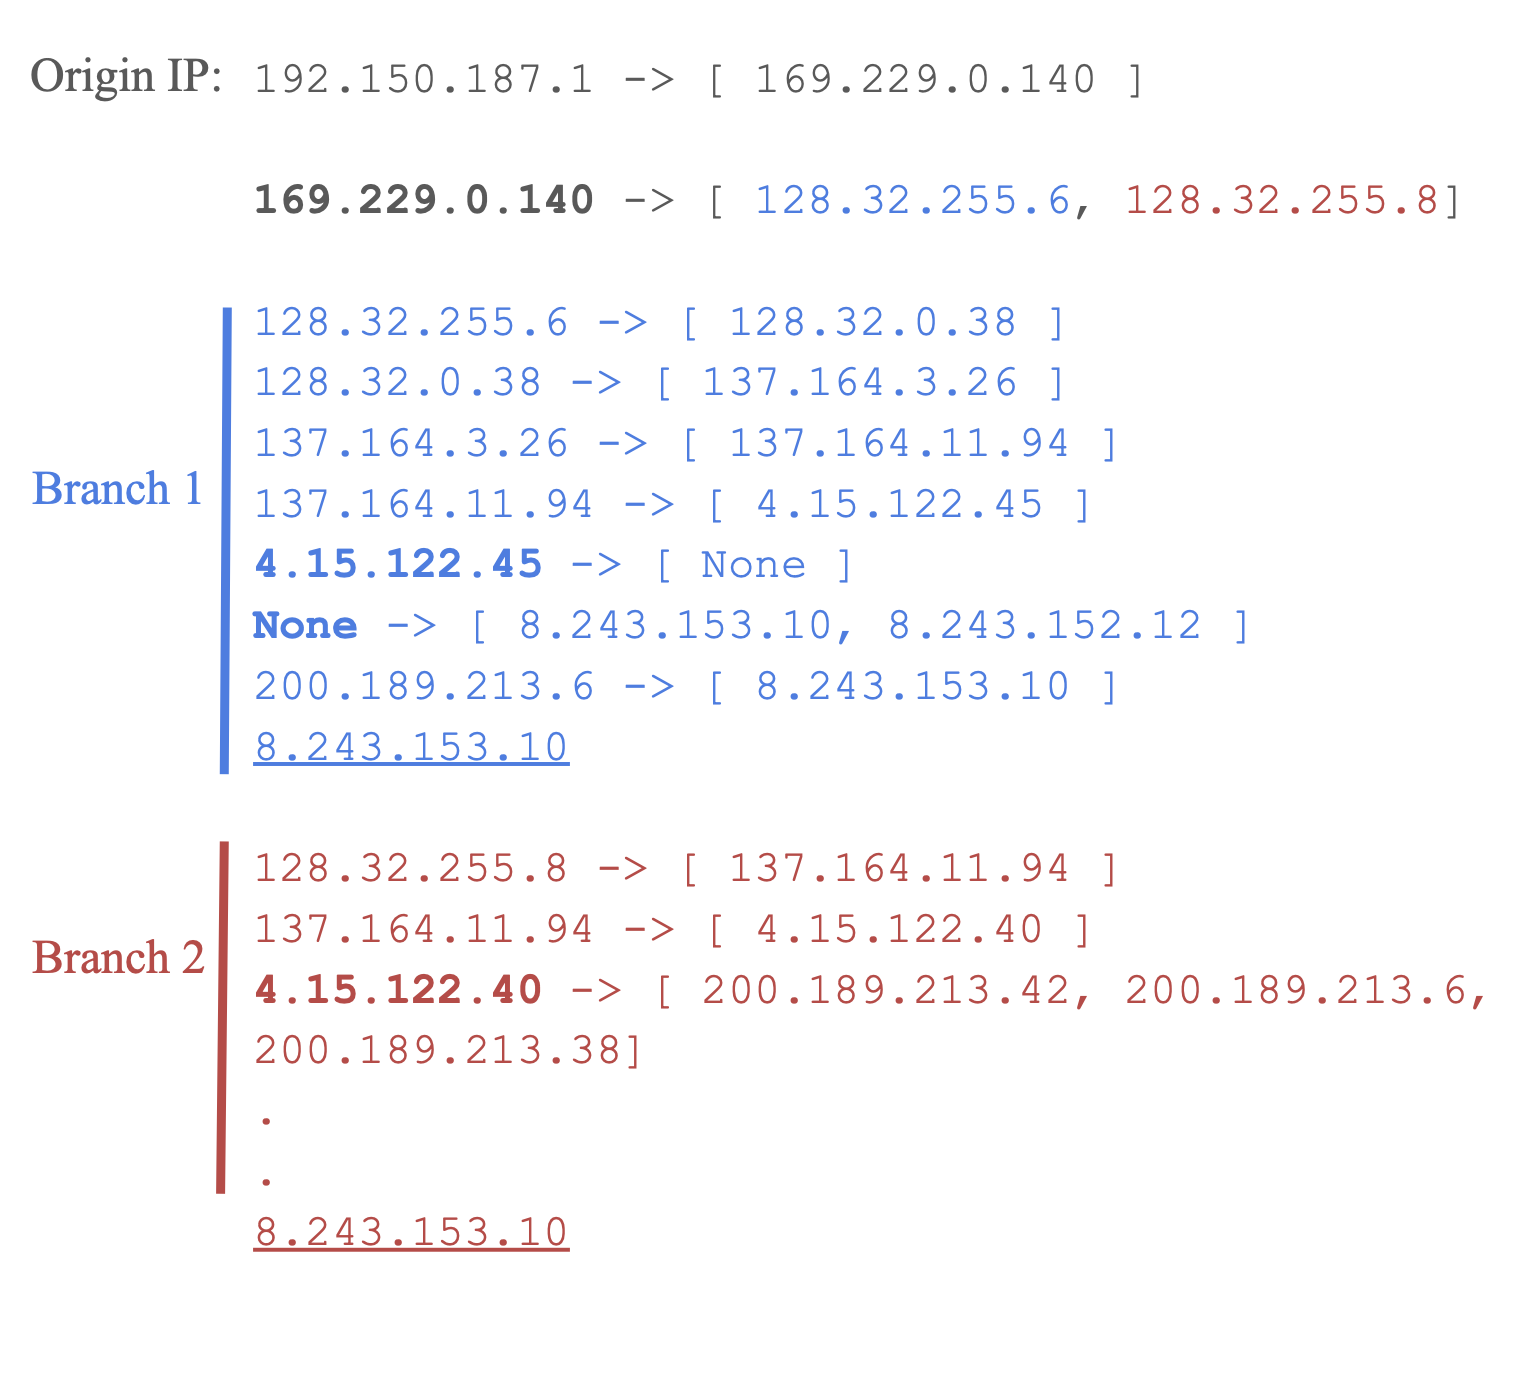
\includegraphics[width=\linewidth]{figures/sample.png}
    \caption{Sample Paris Traceroute Output}
    \label{fig:sample}
\end{figure}


Figure \ref{fig:sample} above is a sample output of a Paris traceroute measurement, detailing the path from a local network to various network nodes. This measurement starts from our origin IP, \texttt{192.150.187.1}, and shows the path it takes to the destination IP, \underline{\texttt{8.243.153.10}}.

Each load balancer encountered along the path is highlighted in bold and creates as many branches as it has next hops. Paris Traceroute then follows each branch, discovering subsequent hops until they converge.

In the figure, the initial load balancer \texttt{169.229.0.140} creates two branches:

\textbf{Branch 1 (Blue):} Starts at the first next hop \texttt{128.32.255.6} and proceeds through several hops. Notably, it includes a hidden next hop, represented as \texttt{None}, which indicates that the IP address is not revealed, possibly due to network policies or configurations that block ICMP responses or other probe packets. This hidden next hop, \texttt{None}, is also a load balancer leading to further hops until the branch reaches the destination \underline{\texttt{8.243.153.10}}. Note that a hidden node can still successfully be identified as a load balancer.

\textbf{Branch 2 (Red):} Starts at the second next hop \texttt{128.32.255.8} and proceeds through several hops. It includes a load balancer \texttt{4.15.122.40} that has three next hops. The branches from these three next hops are simplified for clarity, but they eventually converge to the destination \underline{\texttt{8.243.153.10}}.

Convergence occurs when multiple branches lead to the same destination. In this case, both branches eventually converge at the same IP address, \underline{\texttt{8.243.153.10}}. 

This annotated output represents a typical result from our measurements. While some traces are simpler, others are significantly longer and contain a greater number of load balancers. This example captures most of the special cases we encounter, providing a general overview of the type of data we collect and analyze in our study.
\newpage


\section{Team Cymru IP to ASN List}

An Autonomous System (AS) is a collection of IP networks and routers under the control of a single organization that presents a common routing policy to the Internet. Each AS is assigned a unique identifier known as an Autonomous System Number (ASN), which facilitates the routing of data between different ASes. ASes play a critical role in the overall structure of the Internet, as they help manage the flow of data, ensuring efficient and reliable connectivity across various networks. They are often managed by Internet Service Providers (ISPs), large enterprises, or educational and government institutions.

To map routers to organizations in our analysis, we used the Team Cymru IP to ASN mapping service to resolve IP addresses to their corresponding Autonomous System Numbers (ASNs). Team Cymru maps IP numbers to BGP prefixes and ASNs using data from over 50 Border Gateway Protocol (BGP) feeds, updated every four hours \cite{teamcymru2023ipasn}. Border Gateway Protocol (BGP) is the Internet's primary routing protocol, responsible for exchanging routing information between different ASes on the Internet.

\begin{table}[h]
    \centering
    \begin{tabularx}{0.6\textwidth}{|l|X|}
        \hline
        \textbf{Field} & \textbf{Example} \\
        \hline
        BGP Origin ASN & 23489 \\
        \hline
        BGP Peer ASN & 199.88.100.1 \\
        \hline
        BGP Prefix & 199.88.100.0/24 \\
        \hline
        Prefix Country Code (assigned) & US \\
        \hline
        Prefix Registry (assigned) & arin \\
        \hline
        Prefix Allocation Date & 1994-03-28 \\
        \hline
        ASN Country Code (assigned) & US \\
        \hline
        ASN Registry (assigned) & arin \\
        \hline
        ASN Allocation Date & 1994-03-28 \\
        \hline
        ASN Description & MARINK12, US \\
        \hline
    \end{tabularx}
    \caption{BGP and ASN Information from team Cymru data}
    \label{tab:bgp_asn_info}
\end{table}
 
 We collected ASN-to-IPv4 address information from Team Cymru every month, with their permission. This list was used to cross-reference the IPs identified as load balancers, their next hops, and their destination IPs, providing detailed insights into the load balancers discovered. Table \ref{tab:bgp_asn_info} shows the fields we obtain for each IP address, detailing data about  the Autonomous System it belongs to. 



\section{Ethical Considerations}

This research adhered to strict ethical standards to ensure no harm was caused during data collection. We performed active measurements with care, ensuring they did not overflood the network. We ran only the two necessary probes in parallel to prevent any network disruptions. Additionally, no personal information was collected in our data. Ethical considerations were followed based on the recommendations in  \cite{partridge2016ethical}.



\chapter{Data Analysis}

In this chapter, we examine the distribution and prevalence of load balancers in our previously described Top-2000 and Rand-2000 datasets.

Before presenting the data, it is important to note the exclusion of data from the University of California, Berkeley (UCB). Our measurement vantage point is the International Computer Science Institute (ICSI), which is connected to the Internet via UCB. UCB employs an internal load balancer detected in every Paris Traceroute measurement. While this highlights the use of load balancers in enterprise networks, it does not provide meaningful data about global load balancing trends.

To avoid bias in our analysis and provide a clearer picture of global load balancer utilization, we have excluded this local data. This ensures that our findings are more representative of global Internet trends, rather than being influenced by specific local network conditions at UCB.

\section{Load Balancer Distribution}

The datasets analyzed cover data collected over 116 days from November 9, 2023, to April 16, 2024. The Top-2000 dataset reveals that the number of domains with at least one load balancer ranges from 81 to 1482 domains. The average is 1438.71, and the median is 1463, indicating that on average, roughly \textbf{72\%} of Top-2000 paths include load balancers.

Conversely, the Rand-2000 dataset, spanning 111 days within the same period, shows that the number of domains with load balancers ranges from 994 to 1094. The average is 1046.68, and the median is 1046, indicating that on average, roughly \textbf{52\%} of Rand-2000 paths include load balancers. 

\begin{table}[h]
\centering
\begin{tabular}{|l|c|c|}
\hline
\textbf{Metric} & \textbf{Top-2000} & \textbf{Rand-2000} \\
\hline
Minimum & 81 & 994 \\
\hline
25th Percentile & 1453 & 1035 \\
\hline
50th Percentile (Median) & 1463 & 1049 \\
\hline
75th Percentile  & 1471 & 1059 \\
\hline
Maximum & 1482 & 1094 \\
\hline
Standard Deviation & 149.64 & 16.91 \\
\hline
\end{tabular}
\caption{Statistical Overview of Load Balancer Usage}
\label{tab:stats_overview}
\end{table}

Table \ref{tab:stats_overview} summarizes the key statistics for both datasets. We can see that the number of load balancers remains relatively stable over time for both datasets, with minor fluctuations largely due to outliers. These outliers were typically caused by machine crashes or code-related errors, rather than significant changes in network infrastructure or traffic patterns.













\section{Analysis of Next Hops After Load Balancers}

We focus on understanding the behavior of next hops after load balancers to gain insights into how load distribution is managed across various domains. 

We find 192,357 load balancers in the Top-2000 dataset. The analysis shows that the number of next hops after a load balancer ranges from 2 to 102, with an average of approximately 3.9. This indicates a moderate level of load distribution across multiple paths. The median value is 3, suggesting that half of the load balancers distribute to either three or fewer next hops. The standard deviation, at 5.8, points to significant variability in the number of next hops. The 75th percentile stands at 5, while the 95th percentile reaches 13.

In comparison, the Rand-2000 dataset includes 140,144 load balancers, where the number of next hops ranges from 2 to 25. The average number of next hops is 2.6, suggesting that more than half of the load balancers distribute to only two next hops. This dataset shows lower variability with a standard deviation of 1.3. The 75th percentile is 2, and the 95th percentile is 3, indicating that most load balancers in this dataset are simpler, primarily distributing to 2 or 3 next hops, with some outliers having up to 25.

\begin{table}[h]
\centering
\begin{tabular}{|l|c|c|c|c|c|}
\hline
\textbf{Dataset} & \textbf{Min} & \textbf{Max} & \textbf{Average} & \textbf{Median} & \textbf{Standard Deviation} \\
\hline
Top-2000 & 2 & 102 & 3.9 & 3 & 5.8 \\
Rand-2000 & 2 & 25 & 2.6 & 2 & 1.3 \\
\hline
\end{tabular}
\caption{Statistical Overview of Next Hop Distribution After Load Balancers}
\label{tab:next_hop_stats}
\end{table}

This analysis highlights the differences in load balancing complexity between the datasets, reflecting the broader range of load distribution strategies and setups in environments with varying traffic loads and requirements.

\begin{figure}[h]
    \centering
    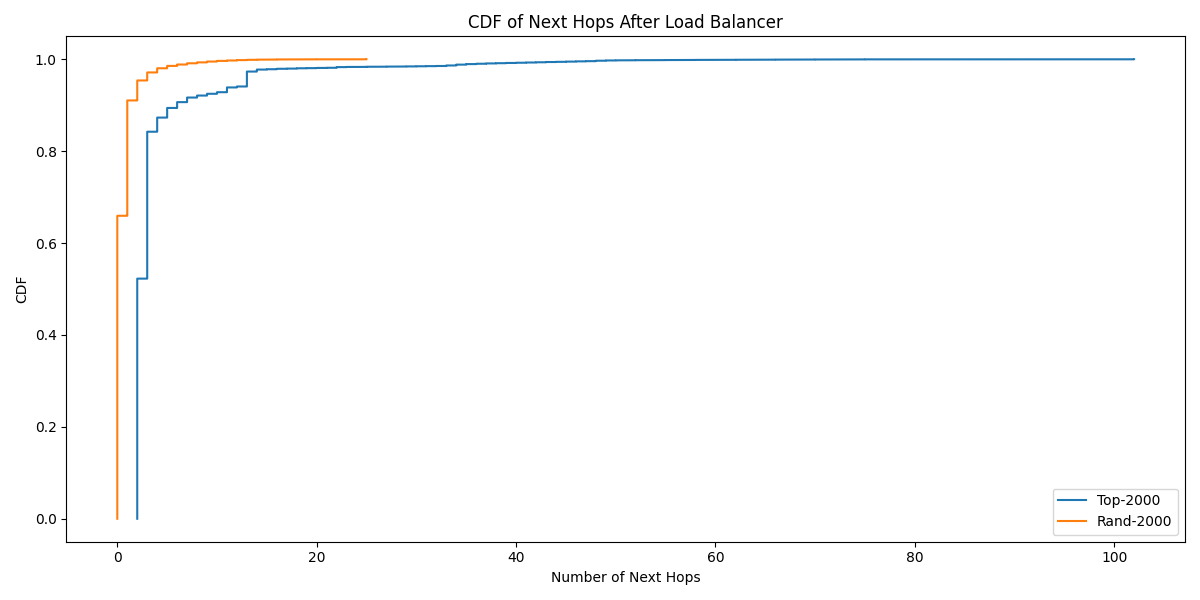
\includegraphics[width=\linewidth]{figures/cdf_next_hops.png}
    \caption{CDF of Next Hops After Load Balancers for Top-2000 and Rand-2000 Datasets}
    \label{fig:cdf_next_hops}
\end{figure}

Figure \ref{fig:cdf_next_hops} illustrates the cumulative distribution function (CDF) of the number of next hops after load balancers for both the Top-2000 and Rand-2000 datasets. The CDF provides a visual representation of the distribution and helps in comparing the two datasets. As shown, the Top-2000 dataset demonstrates a wider spread with more load balancers having a higher number of next hops, whereas the Rand-2000 dataset shows a more concentrated distribution with most load balancers having fewer next hops.

The differences in the number of next hops between the two datasets highlight the varying network configurations and load distribution strategies. The higher variability in the Top-2000 dataset suggests a more complex and distributed network structure, indicating the need for more expansive infrastructure due to the higher traffic these sites receive. In contrast, the Rand-2000 dataset's lower variability and fewer next hops suggest a simpler network configuration for less commonly used paths. These findings align with our hypothesis that the most visited websites require more extensive load balancing to manage their significant traffic demands.

\section{Analysis of ASes with Most Next Hops}

We next aim to understand the Autonomous Systems (ASes) with the highest average number of next hops.  This reveals significant insights into the infrastructure and load balancing at an organizational level.
The ASes with the most next hops typically indicate a robust infrastructure with a greater need for load balancing. This could be due to a high volume of traffic, requiring efficient distribution across multiple servers to avoid bottlenecks, or due to specific requirements such as traffic filtering based on the source. Table \ref{tab:top2000_as_next_hops} shows the ASes that own the load balancers with the most next hops accross top-2000. While table \ref{tab:rand2000_as_next_hops} shows the data for rand-2000. The AS names come directly from the Cymru list. \\
 \\
\begin{table}[h!]
    \centering
    \begin{tabularx}{\textwidth}{|X|r|r|}
        \hline
        \multicolumn{3}{|c|}{\textbf{Top 10 ASes by Average Number of Next Hops (Top-2000)}} \\
        \hline
        \textbf{AS} & \textbf{AS \#} & \textbf{Avg Next Hops} \\
        \hline
        ORACLE-BMC-31898, US & \textbf{31898} & 90.7 \\
        FACEBOOK, US & \textbf{32934} & 25.0 \\
        GOOGLE, US & 15169 & 24.2 \\
        ADJUST-, DE & 205184 & 20.6 \\
        CHINA169-BJ Unicom Beijing, CN & \textbf{4808} & 19.8 \\
        CHINANET-AP, China Telecom, CN & \textbf{23724} & 15.4 \\
        CLOUDFLARENET, US & 13335 & 14.0 \\
        ALIBABA-CN-NET Alibaba Ads, CN & 37963 & 13.9 \\
        CHINANET-SCIDC-AS-AP, CN & \textbf{38283} & 13.8 \\
        CHINANET-BACKBONE No.31, CN & \textbf{4134} & 13.7 \\
        \hline
    \end{tabularx}
    \caption{Top 10 ASes by Average Number of Next Hops for Top-2000}
    \label{tab:top2000_as_next_hops}
\end{table}\newpage

\begin{table}[h!]
    \centering
    \begin{tabularx}{\textwidth}{|X|r|r|}
        \hline
        \multicolumn{3}{|c|}{\textbf{Top 10 ASes by Average Number of Next Hops (Rand-2000)}} \\
        \hline
        \textbf{AS} & \textbf{AS \#} & \textbf{Avg Next Hops} \\
        \hline
        ORACLE-BMC-31898, US & \textbf{31898} & 23.0 \\
        FACEBOOK, US & \textbf{32934} & 7.9 \\
        CHINA169-BJ Unicom Beijing, CN & \textbf{4808} & 6.8 \\
        CHINANET-SH China Telecom, CN & 134768 & 5.2 \\
        ADJUST-, DE & 205184 & 4.4 \\
        CHINANET-SCIDC-AS-AP, CN & \textbf{38283} & 3.3 \\
        CT-IDC No.287, Jin-rong Street, CN & 24353 & 3.0 \\
        CHINANET-BACKBONE No.31, CN & \textbf{4134} & 2.8 \\
        CT-HANGZHOU-IDC No.288, CN & 58461 & 2.3 \\
        CHINANET-BJ-AP, China Telecom, CN & \textbf{23724} & 2.2 \\
        \hline
    \end{tabularx}
    \caption{Top 10 ASes by Average Number of Next Hops for Rand-2000}
    \label{tab:rand2000_as_next_hops}
\end{table}

The order of ASes has many similarities across both datasets, suggesting that larger ASes with more budget tend to develop their infrastructure and add many next hops to their load balancers. This means that even if an AS already has a lot of infrastructure, it remains prevalent even in the less popular paths. Notably, \textit{ORACLE-BMC-31898}, \textit{FACEBOOK}, \textit{CHINA169-BJ Unicom Beijing}, \textit{CHINANET-BJ-AP, China Telecom}, \textit{CHINANET-SCIDC-AS-AP}, and \textit{CHINANET-BACKBONE No.31} appear in both lists, highlighting that 7 of the top 10 ASes are the same in both datasets.



We see a significant presence of Chinese load balancers. According to Bhaskar et al.  \cite{bhaskar2021}, some Chinese providers use load balancers to enforce censorship, which may explain their prevalence. Their study found that packet headers, such as source IP address and source port, can influence DNS censorship. They discovered that 37\% of IPs across 56\% of ASes show changes in censorship behavior based on these parameters. This means that Chinese load balancers are used not only for load distribution but also to control access to information, demonstrating their dual role in managing traffic and enforcing censorship.

In the Rand-2000 dataset, the top 7 to 10 ASes have an average number of next hops below three. Since the minimum is two, these numbers aren't as significant, indicating that most load balancers in this range are of similar rank and complexity.

Despite the similarities in the order of ASes, the Top-2000 dataset shows higher numbers of next hops due to the higher average usage and need for more extensive load balancing. This underscores the importance of expansive infrastructure for the most visited websites, which require robust load balancing solutions to manage their significant traffic demands.

\newpage
\section{Analysis of Next Hop ASes Matches and Mismatches}

The next section examines how often load balancers and their next hops belong to the same Autonomous System (AS) and the implications of matching and non-matching pairs.

Table~\ref{tab:summary_data} presents a detailed summary of the data, showing the total counts for load balancers across different categories of match-mismatch scenarios.\\

\begin{table}[h!]
\centering
\begin{tabular}{|l|c|c|}
\hline
\textbf{Category} & \textbf{Number of Load Balancers} & \textbf{\%} \\
\hline
Fully Matching & 50,089 & 70.7 \\
Partially Matching & 402 & 0.6 \\
No Matching & 20,308 & 28.7 \\
\hline
Total Unique Load Balancers & 70,799 & 100 \\
\hline
\end{tabular}
\caption{Summary of Load Balancer Matching Statistics}
\label{tab:summary_data}
\end{table}
 \\ 


Fully matching next hops, where every next hop AS matches the load balancer AS, account for a significant portion of all unique load balancers. This demonstrates that large organizations often manage their network traffic internally. Internal load balancing is not only a coherent strategy but also cost-effective, especially for organizations expecting substantial traffic. Table~\ref{tab:fully_matching} presents the top ASes with fully matching next hops. 

The "Number of Occurrences" column for Tables \ref{tab:fully_matching}, \ref{tab:partially_matching}, and \ref{tab:no_matching} indicates the number of times a load balancer appears with all its next hops either matching, partially matching or not matching.

\begin{table}[h!]
    \centering
    \begin{tabular}{|l|r|r|}
        \hline
        \multicolumn{3}{|c|}{\textbf{Top 10 ASes with Fully Matching Next Hops}} \\
        \hline
        \textbf{AS} & \textbf{AS \#} & \textbf{Number of Occurrences} \\
        \hline
        Google, US & 15169 & 13,516 \\
        ChinaNet Backbone No.31, CN & 4134 & 6,420 \\
        Comcast-7922, US & 7922 & 5,460 \\
        China169-BJ China Network , CN & 4808 & 4,028 \\
        KDDI Corporation, JP & 2516 & 3,204 \\
        Facebook, US & 32934 & 2,321 \\
        Microsoft-Corp-MSN-AS-Block, US & 8075 & 2,260 \\
        Cogent-174, US & 174 & 1,769 \\
        KIXS-AS-KR Korea Telecom, KR & 4766 & 1,744 \\
        CLOUDFLARENET, US & 13335 & 1,290 \\
        \hline
        \textbf{Total} & & 42,012 \\
        \hline
    \end{tabular}
    \caption{Top 10 ASes with Fully Matching Next Hops}
    \label{tab:fully_matching}
\end{table}
  \newpage
Partially matching next hops, where at least one but not all next hops match the load balancer AS, suggest a mixed routing strategy. This approach might optimize some paths within the AS while others diverge to external networks. Table~\ref{tab:partially_matching} details the top ASes with partially matching next hops. However, the number of load balancers with partially matching next hops is negligible.

\begin{table}[h!]
    \centering
    \begin{tabular}{|l|r|r|}
        \hline
        \multicolumn{3}{|c|}{\textbf{Top 10 ASes with Partially Matching Next Hops}} \\
        \hline
        \textbf{AS} & \textbf{AS \#} & \textbf{Number of Occurrences} \\
        \hline
        ChinaNet-IDC-BJ-AP IDC CN & 23724 & 158 \\
        ChinaNet Backbone No.31, CN & 4134 & 125 \\
        RelianceJio-IN Reliance , IN & 55836 & 30 \\
        Yandex, RU & 13238 & 18 \\
        GlobalDC, FI & 2527 & 17 \\
        Level3, US & 3356 & 15 \\
        NL-Gigapop, US & 2737 & 12 \\
        HiNetUSA HiNet , TW & 3462 & 12 \\
        Alibaba-CN-Net Ads, CN & 37963 & 4 \\
        Alibaba-CN-Net-US , CN & 45102 & 4 \\
        \hline
        \textbf{Total} & & 402 \\
        \hline
    \end{tabular}
    \caption{Top 10 ASes with Partially Matching Next Hops}
    \label{tab:partially_matching}
\end{table}


Next hops with no matching AS comprise a smaller percentage than the fully matching category. When the load balancer AS does not match any next hop AS, it suggests the use of external load balancing services. Table~\ref{tab:no_matching} lists the top ASes with no matching next hops.

\begin{table}[h!]
    \centering
    \begin{tabular}{|l|r|r|}
        \hline
        \multicolumn{3}{|c|}{\textbf{Top 10 ASes with No Matching Next Hops}} \\
        \hline
        \textbf{AS} & \textbf{AS \#} & \textbf{Number of Occurrences} \\
        \hline
        CONE, US & 4685 & 6,908 \\
        Cogent-174, US & 174 & 2,580 \\
        ChinaNet Backbone No.31, CN & 4134 & 2,440 \\
        ChinaNet-IDC-BJ-AP IDC, CN & 23724 & 854 \\
        Level3, US & 3356 & 849 \\
        Yahoo-1, US & 10310 & 608 \\
        CSUNET-NE, US & 2152 & 312 \\
        Google, US & 15169 & 216 \\
        BTN-ASN, US & 14618 & 207 \\
        CT-HANGZHOU-IDC No.288, CN & 58461 & 205 \\
        \hline
        \textbf{Total} & & 15,179 \\
        \hline
    \end{tabular}
    \caption{Top 10 ASes with No Matching Next Hops}
    \label{tab:no_matching}
\end{table}

Overall, while a majority of load balancers manage traffic within their own AS, the presence of partial and no matches suggests a diverse range of load balancing strategies.

In the case of no matching, it is possible that entities like CyrusOne (CONE) and Cogent, which are major players in the data center and ISP sectors respectively, might have connections to multiple other ISPs. This setup allows them to balance loads across these connections to enhance network robustness. No matching could also potentially mean that ISPs are offering load balancing services to smaller data centers or their clients. While ChinaNet load balancers do show up in the no matching category, they are not the dominant presence there. Instead, ChinaNet is more frequently observed in the matching load balancers category. This suggests that despite potential involvement in censorship, ChinaNet predominantly employs its load balancing capabilities to manage internal network traffic.


\newpage
\section{Change Over Time}

This section investigates how load balancing changes over time for the Top-2000 and Rand-2000 datasets, including the total number of days observed, the average daily changes, and the number of reappearances. 

\begin{figure}[h!]
\centering
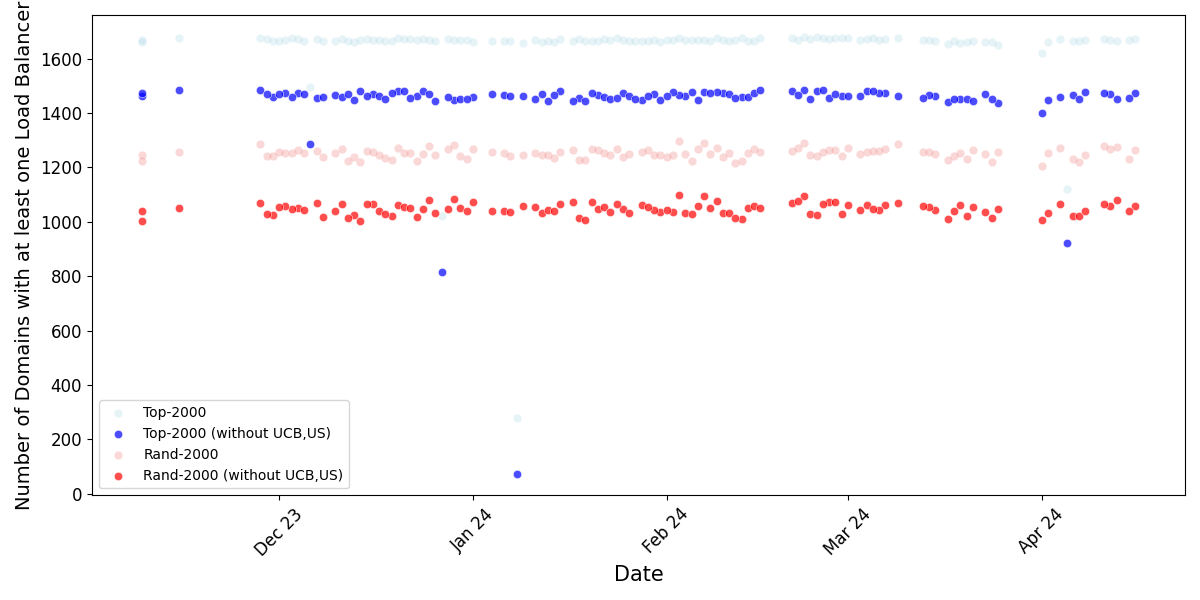
\includegraphics[width=\textwidth]{figures/scatter_plot_domains.png}
\caption{Number of Domains with at least one Load Balancer Over Time}
\label{fig:stat_plot}
\end{figure}

Figure~\ref{fig:stat_plot} shows the number of domains with at least one load balancer over time for both datasets. The plot reveals that, except for some outliers—due to the machine crashing or encountering code-related issues—the amount of load balancing found is quite consistent across time. For days without any records, the machine was completely down for maintenance reasons. This consistency shows the prevalence of load balancers in the global network. However, this consistency is achieved through a dynamic balance of additions and removals as we will discuss next.\\

To understand the dynamics of load balancers over time, we look more granularly at daily changes, including the addition and removal of load balancers. "Added" load balancers refer to those that are not present in the dataset from the previous day but appear in the current day's list. Conversely, "lost" load balancers are present in the dataset on the previous day but do not appear in the current day's list. This dynamic illustrates the fluctuation and turnover within the dataset, showing how frequently load balancers enter and exit the observation scope.

We also find it necessary to note that the observed changes in load balancer presence over time may be influenced by the resolution of hostnames to their current IP addresses, as discussed in \ref{subsec:freq}. The dynamic nature of IP address allocation and the reliance on real-time data from domain name services could result in variations that are not solely indicative of load balancer behavior but also of changes in IP address mappings. This potential artifact should be considered when interpreting the fluctuations and churn of load balancers within the datasets.

%%%@@@ Mark's version of the above ...

%% We note that in this work we report that there is some churn in
%% the load balancers presence between subsequent days.  However, we
%% do not delve into what causes this churn.  The observed changes
%% in load balancer presence over time may be influenced by the
%% resolution of hostnames to their current IP addresses, as
%% discussed in \ref{subsec:freq}. The dynamic nature of IP address
%% allocation and the reliance on real-time data from domain name
%% services could result in variations that are not solely
%% indicative of load balancer behavior but also of changes in IP
%% address mappings.  Additionally, changes could be due to anycast
%% routing that sends our probes to different servers on different
%% days.  These potential causes should be considered when
%% interpreting the fluctuations and churn of load balancers within
%% the datasets.  In addition, understanding the reasons behind the
%% load balancer churn is likely a fruitful area for future work.

\textbf{Top-2000 Dataset:} Over the observation period of 116 days, an average of approximately 253 load balancers are added per day, and an average of about 251 load balancers are lost each day. Figure~\ref{fig:top2000_changes} illustrates the daily changes in the number of load balancers for the Top-2000 dataset. The graph shows that the number of removals and additions starts off with less than 100 in the last 15 days of November but then stabilizes at around 250 in December and onwards, which matches the average values mentioned. The dataset also records a total of 82,318 reappearances, indicating the number of times load balancers reappear after having been previously lost. The average duration of presence for a load balancer in this dataset is roughly 31 days.

\begin{figure}[h!]
    \centering
    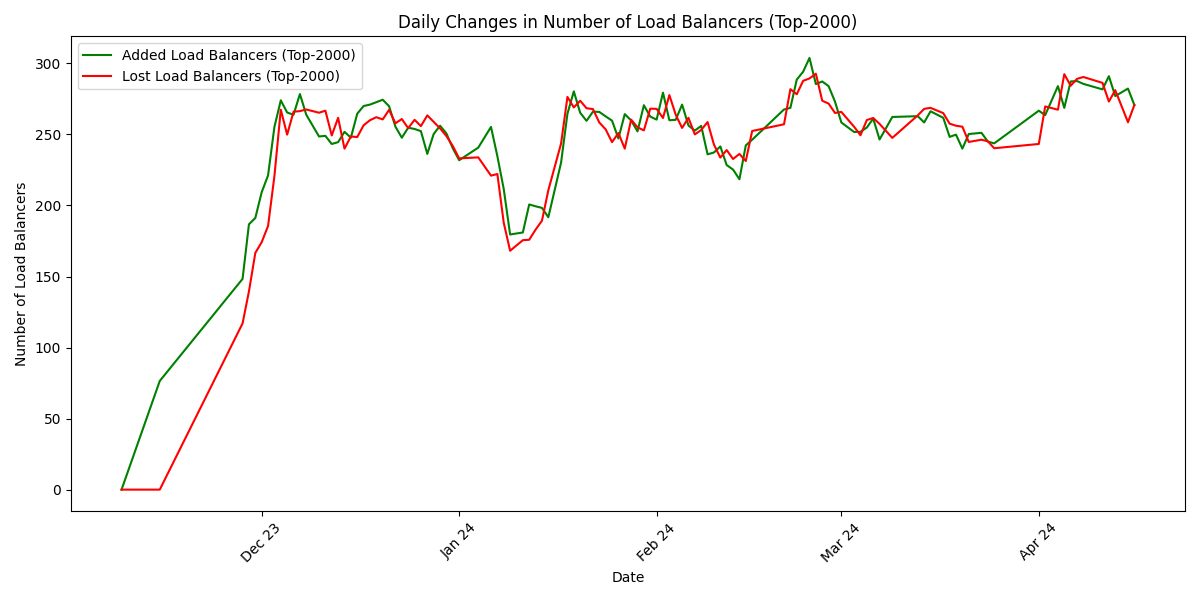
\includegraphics[width=\linewidth]{figures/load_balancer_changes_Top-2000.png}
    \caption{Daily Changes in Number of Load Balancers for Top-2000}
    \label{fig:top2000_changes}
\end{figure}

\textbf{Rand-2000 Dataset:} Similarly, the Rand-2000 dataset, observed over 111 days, shows that on average, approximately 161 load balancers are added per day, while an average of about 162 load balancers are lost each day. Figure~\ref{fig:rand2000_changes} illustrates the daily changes in the number of load balancers for the Rand-2000 dataset. The graph shows that the number of removals and additions starts off with less than 100  December but then stabilizes at around 150, which matches the average values mentioned. The dataset also records a total of 12,139 reappearances, highlighting the instances where load balancers reappear after being lost. The average duration of presence for a load balancer in this dataset is roughly 12 days.

\begin{figure}[h!]
    \centering
    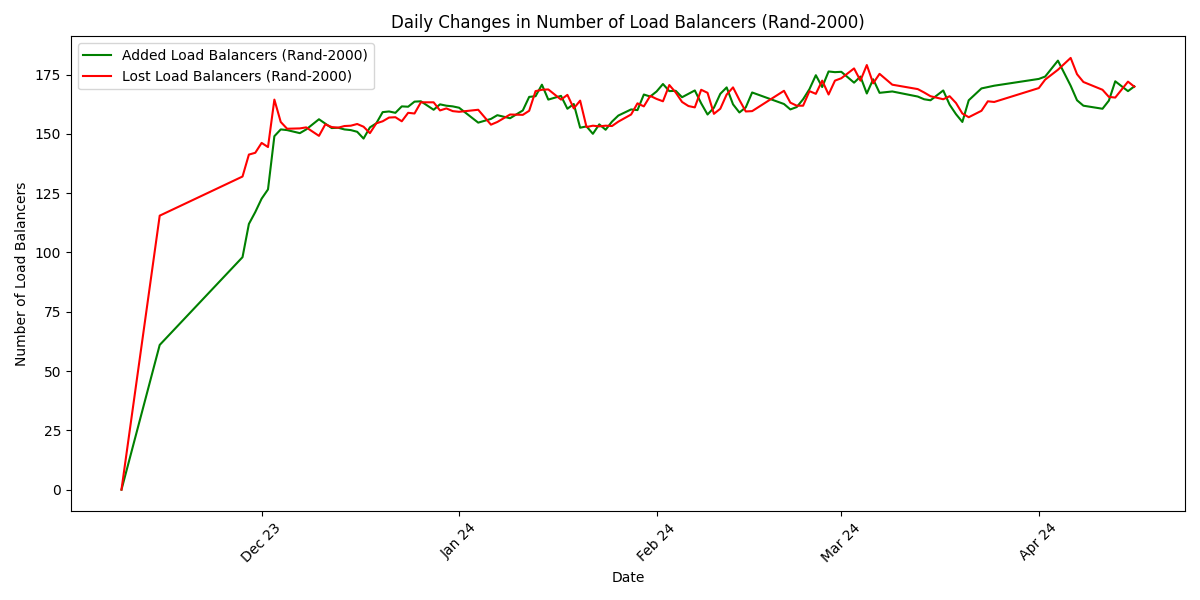
\includegraphics[width=\linewidth]{figures/load_balancer_changes_Rand-2000.png}
    \caption{Daily Changes in Number of Load Balancers for Rand-2000}
    \label{fig:rand2000_changes}
\end{figure}

Both datasets illustrate the dynamic nature of load balancer presence, with frequent entries and exits from the datasets. Initially, the scatter plot in Figure~\ref{fig:stat_plot} suggested a consistent number of load balancers over time. However, the more granular analysis provided by the daily changes in Figures~\ref{fig:top2000_changes} and \ref{fig:rand2000_changes} reveals a dynamic aspect of load balancer behavior. The fact that the number of removals and additions closely matches each day is particularly interesting. This suggests that while the overall network maintains a steady number of load balancers, the specific load balancers performing this function are frequently changing.\\




\begin{figure}[h!]
    \centering
    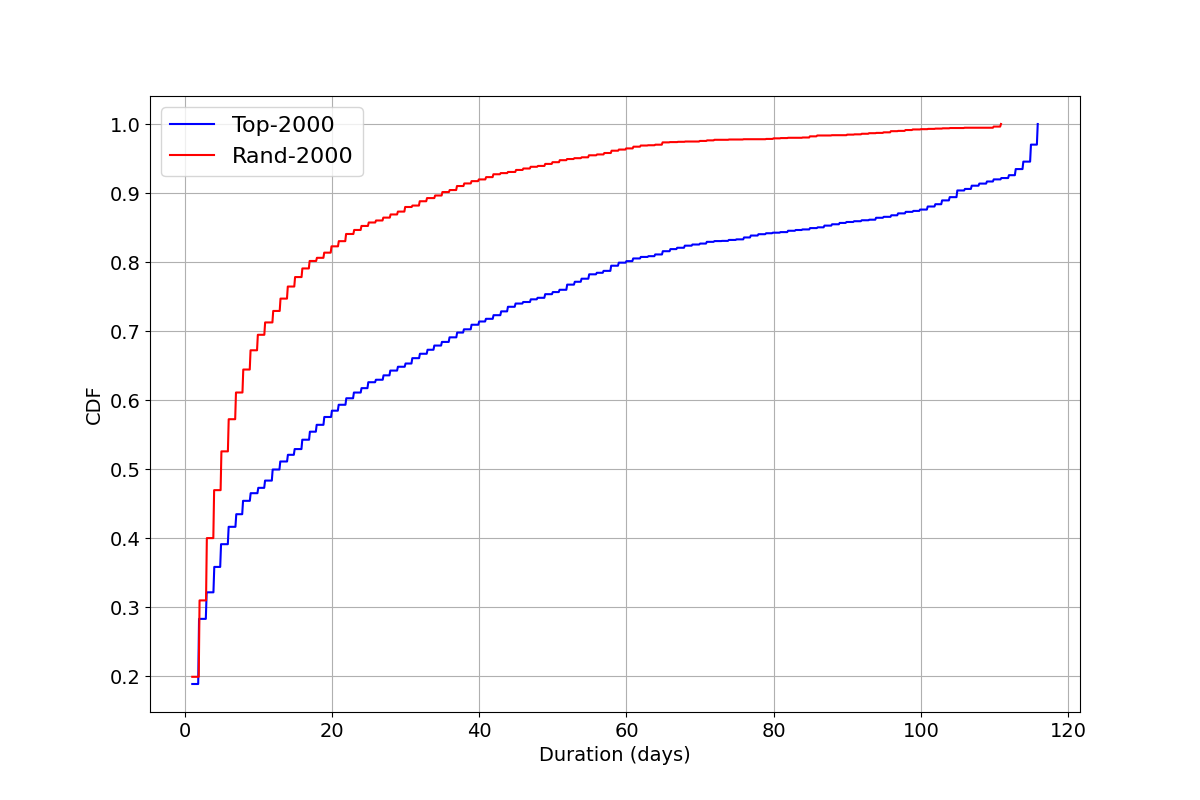
\includegraphics[width=\linewidth]{figures/cdf_load_balancer_durations_comparison.png}
    \caption{Cumulative Distribution Function of Load Balancer Appearances}
    \label{fig:cdf_durations}
\endfigure

To further analyze the consistency of load balancer presence, Figure~\ref{fig:cdf_durations} shows the cumulative distribution function (CDF) for the appearances of load balancers across both datasets. This CDF plot provides insights into the duration that load balancers typically remain active within each dataset. While the operational appearances for the bottom 30\% of the sets are similar, the datasets start to diverge around the 40\% mark. Notably, load balancers in the Top-2000 dataset tend to stay active for longer periods compared to those in the Rand-2000 dataset. This divergence suggests that the most visited sites, typically represented in the Top-2000, maintain their load balancers for longer periods once a path is identified to have high traffic loads. This indicates that there is a longer turnover value for load balancers at highly visited sites. The constant for which a load balancer remains active when introduced to the network seems higher on the most visited sites.

Future work on the presence of load balancers on a more granular hourly basis might reveal whether this dynamic aspect holds true. Such studies could investigate if there is a higher presence of load balancers during peak traffic hours, suggesting that load balancers are actively managed in response to real-time traffic demands.


\section{Change Over Time for Autonomous Systems}

This section presents the Autonomous System (AS)-specific statistics for both the Top-2000 and Rand-2000 datasets, focusing on key metrics that illustrate how each AS manages its load balancing infrastructure over time. These metrics include the daily rate of load balancer additions and removals, indicating the dynamism and adaptability of the infrastructure; the average duration of load balancer presence, suggesting stability; and the consistency of presence, highlighting the reliability of each AS's load management strategy.

We define the following metrics and explore them below:
\begin{itemize}
    \item \textbf{Additions per day}: The average number of load balancers added daily by each AS, suggesting a dynamic response to changing network demands.
    \item \textbf{Removals per day}: The average number of load balancers removed daily by each AS, indicating varying traffic patterns, network updates, or temporary route changes.
    \item \textbf{Average duration of presence}: The average number of days any load balancer from a specific AS remains active, suggesting stability within the network.
    \item \textbf{Consistency}: Measures the AS that had the most vs least amount of change from the beginning to the end of the measurement period, indicating reliability and operational stability. We calculate using the percent change from December 1st, to April 16th, while also looking at middle values to check for outliers. 
    
    \item \textbf{Fluctuation}: Indicates the number of times a single load balancer from a specific AS reappeared. A high fluctuation suggests a high level of dynamism and potential adaptation to network requirements or changing traffic conditions, while a low fluctuation does not necessarily indicate non-adaptability but rather that reappearances are rare.
\end{itemize}


To further clarify the metrics analyzed, each AS can have multiple unique load balancers listed in our dataset. When any of these load balancers is added or removed, it contributes to the total count for that AS in the respective category. Consistency is now defined as the AS that had the most vs least amount of change from the beginning to the end of the measurement period. Fluctuation is now a more predictable version of inconsistency, characterized by frequent changes but often with a discernible pattern, as opposed to inconsistency which lacks a regular pattern or stability.

For the Top-2000 dataset, observed over 116 days, Table~\ref{tab:top-2000-stats} shows statistics for the whole dataset while Table~\ref{tab:top-2000-highest} highlights the ASes with the highest values in various categories.

\begin{table}[h!]
    \centering
    \begin{tabular}{|l|r|r|r|r|}
        \hline
        \textbf{Metric} & \textbf{Avg} & \textbf{25th \%ile} & \textbf{75th \%ile} & \textbf{99th \%ile} \\
        \hline
        \# Additions/day & 6.2 & 3.0 & 15.0 & 50.2 \\
        \hline
        \# Removals/day & 6.2 & 2.0 & 12.5 & 50.1 \\
        \hline
        Duration of presence & 7.4 days & 0.3 days & 13.6 days & 39.0 days \\
        \hline
        Consistency & 4293.0 & 34.3 & 1820.5 & 65867.6 \\
        \hline
        Fluctuation & 450.3 & 4.3 & 712.0 & 6615.7 \\
        \hline
    \end{tabular}
    \caption{Top-2000 Dataset Statistics}
    \label{tab:top-2000-stats}
\end{table}


\begin{table}[h!]
    \centering
    \begin{tabular}{|l|l|r|}
        \hline
        \textbf{Metric} & \textbf{AS with Highest Value (ASN)} & \textbf{Value} \\
        \hline
        Most additions/day & Facebook, US (32934) & 50.3 \\
        \hline
        Most removals/day & CSUNET-NW, US (2152) & 50.2 \\
        \hline
        Longest duration in days & CHINANET-BKBN-31, CN (4134) & 59.6 \\
        \hline
        Most consistent AS in \% & Google, US (15169) & 0.9 \\
        \hline
        Most inconsistent AS in \% & ORACLE-BMC, US (31898) & 26.1 \\
        \hline
        Most fluctuating AS & CHINANET-BKBN-31, CN (4134) & 11,660 \\
        \hline
    \end{tabular}
    \caption{Top-2000 Dataset Highest Values}
    \label{tab:top-2000-highest}
\end{table} 

Table~\ref{tab:top-2000-highest} highlights the ASes with the highest values in various categories. For instance, Facebook, US shows the highest rate of additions per day at 50.3, which is significantly higher than the average of 6.2 additions per day and accounts for 25\% of all additions. Despite this high rate of additions, Facebook only accounts for 18\% of removals, resulting in a net 15\% increase in Facebook load balancers over the four months observed.

In contrast, CSUNET-NW, US shows the highest rate of removals per day at 50.2, which also accounts for 25\% of all removals. However, CSUNET-NW's removals stabilized over time, resulting in only a 5\% decrease in their load balancers between the first and last day of measurment.

The longest duration of presence is observed in CHINANET-BACKBONE No.31, CN at 59.6 days, indicating a very stable and long-term presence compared to the average of 7.4 days. Most ASes with high duration values are based in the US, with the second highest duration being 40 days, 19 days less than CHINANET-BACKBONE. 

Google, US emerges as the most consistent AS with minimal changes observed over the observation period a 0.9\% change over the measurement period as well as over the midpoint days. 

Conversely, ORACLE-BMC-31898, US is noted as the most inconsistent AS with 26.1\% net increase over our measurement period with a steady increase over time.

CHINANET-BACKBONE No.31, CN is the most fluctuating AS with 11,660 instances of reappearance. Some load balancers sporadically appeared and disappeared, while others remained for a long enough period of time to have the longest average duration of presence.




For the Rand-2000 dataset, observed over 111 days, Table~\ref{tab:rand-2000-stats} displays the average, 25th percentile, 75th percentile, and 99th percentile values for each metric. Table~\ref{tab:rand-2000-highest} lists the ASes with the highest values in various categories.

\begin{table}[h!]
    \centering
    \begin{tabular}{|l|r|r|r|r|}
        \hline
        \textbf{Metric} & \textbf{Avg} & \textbf{25th \%ile} & \textbf{75th \%ile} & \textbf{99th \%ile} \\
        \hline
        \# Additions/day & 14.1 & 0.8 & 16.3 & 21.6 \\
        \hline
        \# Removals/day & 15.2 & 0.8 & 22.5 & 21.4 \\
        \hline
        Duration of presence & 2.3 days & 0.1 days & 4.1 days & 30.7 days \\
        \hline
        Consistency & 702.2 & 9.0 & 1920.1 & 10375.1 \\
        \hline
        Fluctuation & 309.3 & 15.8 & 473.8 & 4290.2 \\
        \hline
    \end{tabular}
    \caption{Rand-2000 Dataset Statistics}
    \label{tab:rand-2000-stats}
\end{table}

Table~\ref{tab:rand-2000-stats} provides an overview of the Rand-2000 dataset. The average and percentile values for additions, removals, and duration indicate that the Rand-2000 dataset experiences more modest changes compared to the Top-2000 dataset. The lower consistency and fluctuation values suggest a less dynamic but more varied infrastructure.

\begin{table}[h!]
    \centering
    \begin{tabular}{|l|l|r|}
        \hline
        \textbf{Metric} & \textbf{AS with Highest Value} & \textbf{Value} \\
        \hline
        Most additions/day & CHINANET-31, CN (4134) & 29.1 \\
        \hline
        Most removals/day & FACEBOOK, US (32934) & 29.4 \\
        \hline
        Longest duration in days & CSUNET-NW, US (2152)& 44.1 days \\
        \hline
        Most consistent AS in \% & GOOGLE, US (15169)& 0.5\% change \\
        \hline
        Most inconsistent AS in \% & COMCAST-7922, US (7922) & -31.6\% \\
        \hline
        Most fluctuating AS & CHINANET-31, CN (4134) & 6,495 \\
        \hline
    \end{tabular}
    \caption{Rand-2000 Dataset Highest Values}
    \label{tab:rand-2000-highest}
\end{table}

Table~\ref{tab:rand-2000-highest} lists the ASes with the highest values in various categories.

CHINANET-BACKBONE No.31, CN shows the highest rate of additions per day at 29.1, accounting for 19.1\% of all additions, but also has a high rate of removals at 29.4, making it overall consistent with a 1.5\% change over the observation period. 

Here, Facebook, US contrasts with the Top-2000 dataset by having an average of 27 additions per day and 29.4 removals per day, resulting in a net decrease in load balancers with an overall change of -5.4\%.

The longest duration of presence is observed in CSUNET-NW, US at 44.1 days. A value of 44.1 is less of an outlier compared to the Top-2000 dataset, with the second longest duration being 35.1 days.

Google, US is the most consistent AS across both datasets with a minimal change of 0.5\%, highlighting its prevalence and the high levels of traffic it consistently handles.

COMCAST-7922, US is the most inconsistent AS with a -31.6\% change. This high inconsistency resulted in an overall decrease in the number of load balancers, with an average of 10 removals per day and only 4 additions per day.

CHINANET-BACKBONE No.31, CN is again the most fluctuating AS with 6,495 instances of reappearance. Some load balancers sporadically appeared and disappeared, while others remained for long enough periods to have the longest average duration of presence.

Overall, there are some notable similarities and differences between the Top-2000 and Rand-2000 datasets. Google, US is consistently the most stable AS across both datasets, highlighting its critical role in handling high volumes of traffic. CHINANET-BACKBONE No.31, CN is the most fluctuating AS in both datasets, indicating its dynamic nature in managing load balancers. However, Facebook, US shows a contrasting behavior between the datasets, with a net increase in load balancers in the Top-2000 dataset and a net decrease in the Rand-2000 dataset. This difference suggests varying strategies or demands across different segments of the Internet. 

While the highlighted metrics for these specific ASes are noteworthy, it is important to recognize that these are just the top values and outliers within our dataset. These numbers provide interesting insights but may not represent the overall behavior of the entire network. Nonetheless, the recurring presence of these ASes in our analysis sections suggests that their unique behaviors have significant implications for network performance and reliability. Understanding that these ASes behave differently from the average can help in understanding the network better. Future work could focus on analyzing each specific AS in greater detail to understand their evolutionary patterns and behaviors over time in a more controlled setting.

\newpage



\section{Shared Next Hops Analysis}

This section analyzes the shared next hops between load balancers in both the Top-2000 and Rand-2000 datasets to understand the extent to which next hops are shared among multiple load balancers, indicating the presence of common infrastructure and potential load balancing strategies.

The data in Table~\ref{tab:shared_next_hops_summary} provides a detailed comparison of shared next hops between the two datasets. The Top-2000 dataset shows a higher average number of load balancers sharing the same next hop compared to the Rand-2000 dataset. This suggests that the most visited sites (Top-2000) are more likely to use common infrastructure for load balancing, potentially due to higher traffic demands requiring more robust and interconnected pathways. 

\begin{table}[h!]
    \centering
    \begin{tabular}{|l|r|r|}
        \hline
        \textbf{Metric} & \textbf{Top-2000} & \textbf{Rand-2000} \\
        \hline
        Total Unique Next Hops & 90,492 & 85,797 \\
        Minimum Load Balancers per Next Hop & 1 & 1 \\
        Maximum Load Balancers per Next Hop & 52 & 42 \\
        Average Load Balancers per Next Hop & 5.31 & 3.35 \\
        Median Load Balancers per Next Hop & 2.0 & 2.0 \\
        Standard Deviation & 6.70 & 4.17 \\
        75th Percentile & 7.0 & 4.0 \\
        95th Percentile & 18.0 & 13.0 \\
        \hline
    \end{tabular}
    \caption{Shared Next Hops Statistics in the Top-2000 and Rand-2000 Datasets}
    \label{tab:shared_next_hops_summary}
\end{table}

The high variability in the number of shared next hops in the Top-2000 dataset, with a maximum of 52 load balancers sharing a single next hop, indicates a significant concentration of traffic through certain key points in the network. This could point to the existence of major nodes or hubs that handle large volumes of traffic, suggesting an optimized but potentially riskier infrastructure due to single points of failure.

In contrast, the Rand-2000 dataset, while still showing shared next hops, has a lower average and maximum number of load balancers per next hop. This suggests a more distributed and less interconnected infrastructure, which might be due to the more varied and less predictable traffic patterns of randomly selected websites.


The distribution of shared next hops, as depicted in Figure~\ref{fig:shared_next_hops_combined}, illustrates that most next hops are shared by a relatively small number of load balancers. However, a small subset of next hops in the Top-2000 dataset are highly shared, suggesting a more interconnected infrastructure and the utilization of common pathways more frequently than in the broader, randomly selected websites of the Rand-2000 dataset.

\begin{figure}[h!]
    \centering
    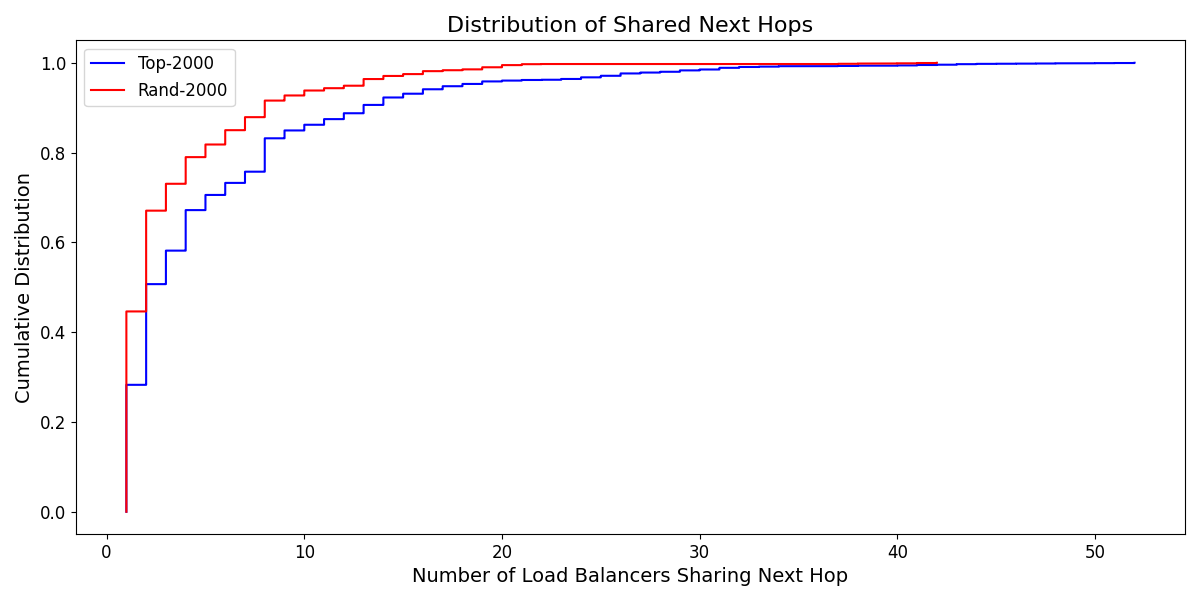
\includegraphics[width=\linewidth]{figures/shared_next_hops_combined.png}
    \caption{Distribution of Shared Next Hops for Top-2000 and Rand-2000}
    \label{fig:shared_next_hops_combined}
\end{figure}

Overall, the presence of shared next hops signifies the use of common infrastructure, which can enhance efficiency but also poses risks in terms of single points of failure. The variability in the number of shared next hops across both datasets underscores the complexity and dynamic nature of load balancing in different segments of the Internet. The more interconnected infrastructure observed in the Top-2000 dataset highlights the necessity for robust load balancing strategies to handle higher traffic loads efficiently.



\chapter{Discovering Hidden Nodes in Cisco Express Forwarding}

In our research, we identified many load balancers within the Internet2 Autonomous System. The Internet2 Network, established to support data-intensive research and academic computing needs, provides tools such as the Internet2 Looking Glass \cite{Internet2_looking_glass}, which allow users to run commands against network devices, enabling testing and viewing active configuration and state information.

The load balancers discovered via Paris Traceroute were also validated through the Internet2 Looking Glass, affirming the effectiveness of our detection methodology. We observed that many of the next hops for these load balancers were defined in Cisco Express Forwarding (CEF) tables. The following sections elaborate on the workings of CEF and its role in load balancing.

\section{Network Layer Load Balancing}

Layer 3, the network layer, performs load balancing by routing packets based on their IP addresses, focusing on traffic distribution across multiple servers without inspecting packet contents. This method is efficient and fast but offers less granularity in traffic management compared to higher-layer solutions, which can make decisions based on the data within the packets. Layer 3 load balancers can efficiently handle large volumes of traffic, they lack the detailed traffic management capabilities provided by higher-layer solutions \cite{zhang}.

\section{Cisco Express Forwarding (CEF)}

Cisco Express Forwarding (CEF) enhances the efficiency of Layer 3 load balancing by pre-computing forwarding information---which sets up where a router sends a packet---based on historical network usage data. CEF uses two primary data structures: the Forwarding Information Base (FIB) and the adjacency table \cite{cisco2017cef}.

The \textbf{Forwarding Information Base (FIB)} is used by CEF to make IP destination prefix-based switching decisions. It is similar to a routing table, maintaining a mirror image of the forwarding information in the IP routing table. When routing changes occur, the IP routing table updates, and these changes are reflected in the FIB, ensuring all known routes are covered without the need for route cache maintenance.

The \textbf{Adjacency Table} stores Layer 2 addressing information necessary for packet forwarding. Nodes in the network that can reach each other with a single hop across a link layer have their Layer 2 next-hop addresses stored in this table. 

When a packet arrives, it is placed into input buffers on the receiver hardware component. The Layer 2/Layer 3 forwarding engine accesses the packet's information and determines its route based on the FIB and adjacency table. The appropriate Layer 2 information is then appended to the packet using data from the adjacency table, and the packet is forwarded to its next-hop destination. CEF also maintains a log of forwarding history to inform future strategies.

\section{Summary and Findings}

Analyzing the Internet2 load balancers reveals that most next hops we found in data collection are defined within CEF. Internet2's load balancing is less resource-intensive, as it does not require deep inspection of packets. The adjacency table is what we can see on the looking glass, not the FIB. When something is moved to the FIB, it becomes an active next hop. However, many next hops found were active in the adjacency table, were not discoverable using our tools.

Our findings suggest that a significant number of load balancers could be hidden in the network because Cisco routers did not see the need to update the FIB with a second next hop. The prevalence of CEF load balancing in the Internet2 network implies that while load balancing may appear dynamic, it is not dynamic in real-time. Instead, CEF learns from previous data for efficiency and does not adapt to specific packet details.

The validation process using the Internet2 Looking Glass confirmed that the load balancers we detected via Paris Traceroute indeed existed in the ground truth as seen through the Looking Glass. However, we weren't able to reach more than 97\% the defined next hops in the adjacency table. We attempt some techniques discover a higher number of next hops in the next section. 


\section{Modifications to the MDA Algorithm}

The number of probes sent out by the Multipath Detection Algorithm (MDA) might have caused an undercount of the load balancers present on the Internet2 network. These values were theoretically derived in the MDA paper. We modified the way it decides how many probes to send. A portion of the probe table used by MDA, which outlines the number of probes needed for varying hop counts, is shown below:

\begin{verbatim}
static const int k[][2] = {
    {   0,   0 }, {   0,   0 }, {   6,   8 }, {  11,  15 },
    {  21,  28 }, {  27,  36 }, {  33,  43 }, {  38,  51 }, 
    ...
    { 712, 866 }, { 720, 876 }, { 729, 886 }, { 737, 896 }, 
};
\end{verbatim}

The values represent the number of probes to send for different hop counts, with the first column indicating probes for a 95\% confidence level and the second column for a 99\% confidence level.

In an attempt more load balancers, we modified the MDA algorithm by multiplying the values in the probe table by 10. This brute-force approach aimed to increase the likelihood of uncovering hidden paths and load balancers. The results show that in some instances, two or three additional load balancers were discovered for some domains. However, the increase in discoverable load balancers was inconsistent, with only about a 2\% average increase. This minor increase does not justify the added cost of such measurements.

Moreover, the increased number of probes significantly extended the measurement duration, taking approximately 20 times longer than standard MDA measurements. This makes the brute-force approach impractical for extended data collection. Interestingly, this approach validates the accuracy of the original MDA probe table, confirming its effectiveness in typical scenarios.

The challenges faced during the enhanced probing trials highlight the limitations of brute-force approaches in discovering hidden load balancers. While increased probes reveal on average 2\% more load balancers, the overall impact was minimal compared to the substantial increase in measurement time. This suggests that simply increasing the number of probes is not the most effective way to uncover hidden load balancers.

Future work could focus on optimizing the probe sending strategy, exploring adaptive probing techniques, and integrating additional contextual information to improve the efficiency of the MDA algorithm. Targeted testing over a longer period could reveal rotations of next hops, and using different types of packets might help uncover more load balancers. These and other potential improvements are discussed in the future works chapter.



\chapter{Summary}
In this study, we investigate the prevalence and characteristics of load balancing on the Internet using comprehensive data collection and analysis. Our research aimed to quantify load balancing behavior providing updated insights into the structure of the modern Internet routing infrastructure.

\section*{Data Collection and Methodology}

In Chapters 3 and 4, we detailed our methodology for data collection, which involved daily measurements from November 2023 to April 2024. We utilized the Alexa Top 1 Million Websites list to select two subsets: the Top-2000 and the Rand-2000 lists. Our measurements were conducted using Paris Traceroute with the Multipath Detection Algorithm (MDA) to identify and classify load balancers. Throughout the study, roughly 450,000 Paris Traceroutes were collected, providing a robust dataset that allows for a relevant quantification of the Internet's load balancing infrastructure.

\section*{Load Balancer Distribution and Trends}

We observed significant trends in load balancer distribution:
\begin{itemize}
    \item The Top-2000 dataset shows a high prevalence of load balancers, with an average of 72\% of paths containing load balancers. The Rand-2000 dataset had 52\%, indicating widespread use across diverse websites. Previous data from \cite{augustin2010measuring} showed that 39\% of paths traversed load balancers, with up to 71\% when considering different types of load balancing. Our data focuses on the most common paths, providing a different perspective. While the site lists are different, we see an overall slight increase of load balancers across all paths explored.
    \item Analysis of next hops shows that popular websites use load balancing structures with more next hops, indicating complexity, while randomly selected sites have simpler configurations with fewer next hops.
    \item Our next hop analysis suggested that the infrastructure supporting the most popular websites is more interconnected and utilizes shared pathways more frequently than the broader, randomly selected websites.
    \item The consistent presence of ASes like GOOGLE, US and CONE,US , in the Top-2000 dataset but their inconsistent presence in the Rand-2000 dataset suggests deliberate adjustments based on traffic expectations. The Top-2000 list likely experiences more predictable high traffic, requiring continuous load balancing, whereas the Rand-2000 list may see more variable traffic patterns, leading to less consistency.
\end{itemize}

\section*{Dynamic and Static Properties}

Our study identified both dynamic and static properties of load balancing:
\begin{itemize}
    \item Load balancers show dynamic behavior, with daily additions and removals reflecting adaptive traffic management. The average presence duration was 31.10 days for the Top-2000 dataset and 12.49 days for the Rand-2000 dataset.
    \item Static properties included the overall number of load balancers discovered for each list. While the load balancers themselves are volatile, load balancing remains constant over time.
    
\end{itemize}

\section*{Layer 3 Load Balancing and Cisco Express Forwarding}

We explored Layer 3 load balancing, focusing on Cisco Express Forwarding (CEF):
\begin{itemize}
    \item CEF optimizes packet forwarding by utilizing pre-computed forwarding information, but does not react to the network condition in real time.
    \item Our analysis of Internet2 load balancers reveals a high reliance on CEF, with many next hops predefined in CEF tables. 
\end{itemize}

\section*{Challenges}

\begin{itemize}
    \item Using Paris Traceroute we were not able to detect all the load balancers in the Internet2 network that we know exist.
    \item Enhanced probing trials using a modified MDA algorithm provided limited success, suggesting the need for more sophisticated techniques.
    \item Future work could focus on adaptive probing methods and integrating contextual information to improve load balancer detection.
\end{itemize}

Overall, our research contributes to a deeper understanding of load balancing on the Internet, highlighting both its complexities and areas for further exploration.

\chapter{Future Work}

There are several areas related to this research that we could not explore because of time or scope constraints. 

\section*{Increasing the Number of Destinations}

One potential for future work is to increase the number of destinations significantly. \textbf{\cite{augustin2010measuring} }conducted measurements from 15 sources to over 68,000 destinations, revealing that many routes pass through load balancers. Given enough time and resources, our goal would be to match or exceed these numbers to get a better understanding of load balancing across the Internet. While our different lists attempted to show an as complete as possible view, higher numbers would ultimately help provide a more complete picture of global traffic patterns.

\section*{Deeper Focus on Autonomous System}
Future research should aim to delve deeper into the specific behaviors and strategies of individual ASes, particularly those that consistently appear as outliers in our analysis. By conducting detailed case studies and longitudinal analyses, we can better understand the factors driving their load balancing strategies and network dynamics. Additionally, expanding the scope to include more datasets and incorporating real-time monitoring could provide a more comprehensive view of AS evolution and help in the development of predictive models for network management. This would enable a more proactive approach to optimizing network performance and enhancing overall Internet stability.

\section*{Adapting MCA to Scamper}

Another area for future research is to adapt the Multipath Classification Algorithm (MCA) to work with Scamper or a new traceroute tool. MCA improves the identification of load balancers by considering different bits in the packet header. Integrating MCA with a tool like Scamper would allow for efficient data collection, similar to the Multipath Detection Algorithm (MDA) and Paris Traceroute. MDA systematically discovers all paths by varying flow identifiers in probe packets. This could help us identify and classify load balancers more accurately and efficiently. 

Additionally, future work could explore the integration of both techniques. Specifically, MDA could be used to get a quick initial assessment of the presence of load balancing. If evidence of load balancing is detected, MCA could then be employed to perform a more detailed analysis. This combined approach would leverage the strengths of both algorithms, offering both efficiency and depth in load balancer detection and classification.


\section*{Per-Flow and Per-Destination Load Balancers}

\textbf{\cite{4261334}} highlighted the importance of distinguishing between per-flow and per-destination load balancers. Per-flow load balancing ensures that all packets in the same flow follow the same path, while per-destination load balancing distributes traffic based on destination IP addresses. Future work could explore these two types of load balancing in more detail, examining how common they are and their impact on network performance. Understanding these differences could help improve network efficiency and reliability.

\section*{Developing Tools for Identifying CEF Load Balancers}

We spent considerable time trying to modify MDA to discover more Cisco Express Forwarding (CEF) load balancers. A future goal could be to develop a tool that can better identify CEF load balancers or detect if some load balancers are hidden. More specifically by conducting targeted measurements over an extended period of time in an attempt to identify additions and removals to the FIB. This would help in providing a more accurate picture of load balancing techniques used in modern networks.

\section*{Assessing the Impact of Load Balancing}

Future work should also focus on assessing the impact of load balancing on network performance. This includes examining whether load balancing techniques improve performance or make it more variable. A study using traceroute combined with web browser performance assessments could provide valuable insights into how load balancing affects the user experience. Understanding the real-world impact of load balancing would help in optimizing network strategies and improving overall performance.

Overall, expanding this research in these directions could provide deeper insights into load balancing on the Internet, helping improve network performance and reliability.

\appendix
\chapter{}

\printbibliography[heading=bibintoc]

\end{document}
